
%***************************************************************************
%
% CreditCruncher - A portfolio credit risk valorator
% Copyright (C) 2004 Gerard Torrent
%
% This program is free software; you can redistribute it and/or
% modify it under the terms of the GNU General Public License
% as published by the Free Software Foundation; either version 2
% of the License.
%
% This program is distributed in the hope that it will be useful,
% but WITHOUT ANY WARRANTY; without even the implied warranty of
% MERCHANTABILITY or FITNESS FOR A PARTICULAR PURPOSE.  See the
% GNU General Public License for more details.
%
% You should have received a copy of the GNU General Public License
% along with this program; if not, write to the Free Software
% Foundation, Inc., 59 Temple Place - Suite 330, Boston, MA 02111-1307, USA.
%
%
% titlepage.tex - TeX documentation file
% --------------------------------------------------------------------------
%
% 2004/12/04 - Gerard Torrent [gerard@fobos.generacio.com]
%   . initial release
%
%***************************************************************************

\def\numversion{0.6}
\def\svnversion{R255:258M}

\title{CreditCruncher - Technical Document \\
Version \numversion\ [\svnversion]\\
\ \\
\centerline{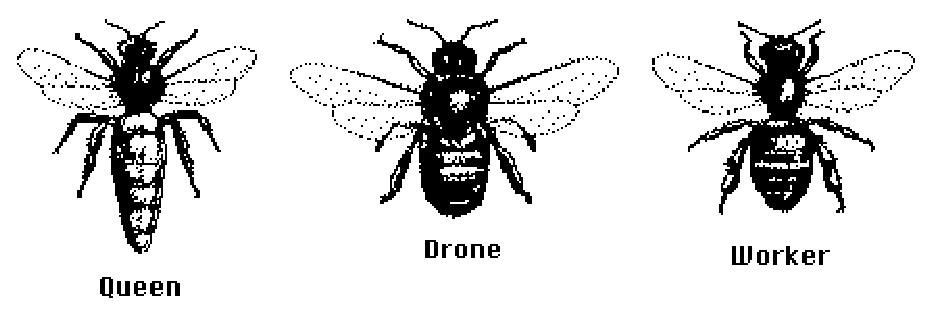
\includegraphics[height=3cm, angle=0]{./images/threebees.eps}}
}

\author{Gerard Torrent Gironella}

\maketitle

\thispagestyle{empty}

\newpage

\vspace*{6in}

\noindent Copyright $\copyright$ 2004-2005 Gerard Torrent Gironella.\\

\noindent The image found in cover have been taken from Mark L. Winston. 1987. 
\emph{The Biology of the Honey Bee} (ISBN: 0-671-07109-2). Harvard University 
Press. Cambridge, MA. These redrawn figures appear here without permission of 
Harvard University Press [Ref: 973029].\\

\noindent This file is part of the CreditCruncher software package.  For
license information, see the COPYING file in the top level directory
of the CreditCruncher source distribution.
